%%%%%%%%%%%%%%%%%%%%%%%%
%
% $Autor: Wings $
% $Datum: 2020-07-24 09:05:07Z $
% $Pfad: GDV/Vortraege/latex - Ausarbeitung/Kapitel/Bezier.tex $
% $Version: 4732 $
%
%%%%%%%%%%%%%%%%%%%%%%%%

\section{Allgemeine mathematische Beschreibung Bézier-Kurve}

Bézier-Kurven werden mit Hilfe von Bernsteinpolynomen gebildet. Wenn mindestens zwei Punkte sowie zwei Tangenten bekannt sind, können Kontrollpunkte ermittelt werden mit denen ein Kontrollpolygon gebildet wird. An diesem Kontrollpolygon  orientiert sich der Verlauf der Kurve. Die Anzahl der  Kontrollpunkte ist abhängig vom Grad der Bézier-Kurve.  Eine Bézier-Kurve vom Grad n hat n+1 Kontrollpunkte.  Die Berechnung der Bézier-Kurve erfolgt über den De-Casteljau-Algorithmus.

\bigskip

\DEF
{
  Im Intervall $[0;\, 1]$ ist das \textbf{ Bernstein-Polynom n-ten Grades}	definiert durch:
	
  \begin{equation}
	b_{i,n}(\lambda) = \binom{n}{i} (1-\lambda)^{n-i} \lambda^{i}, \quad \lambda \in [0,1], \quad i=0,\dots,n
	\label{Bernsteinpolynome}
  \end{equation}
}

\bigskip

\DEF
{
  Der Binomialkoeffizient ist definiert durch:
    
 \begin{equation}
   \binom{n}{i}=\frac{n!}{i!(n-i)!}, \quad i=0, \dots ,n  
   \label{Binomialkoeffizient}
 \end{equation}
}	

\bigskip

Hierbei bilden die Bernstein-Polynome $b_{i,n}$ eine Basis des Vektorraumes $\Po^n(I)$ der Polynome höchstens vom Grad $n$ über $I$. Somit lässt sich jedes Polynom höchstens $n$-ten Grades eindeutig als Linearkombination schreiben.	%P in mathematisch 
\cite{Farin:2002}

\bigskip

\BEISPIEL{
  Bestimmung von Bernstein-Polynome für $n = 3 $ gilt:

  $$
    \begin{array}{*4{>{\displaystyle}c}}
      b_{3,0}(\lambda) &= \binom{3}{0} (1-\lambda)^{3-0} \lambda^{0} &=& (1-\lambda)^{3}\\  \\
      b_{3,1}(\lambda) &= \binom{3}{1} (1-\lambda)^{3-1} \lambda^{1} &=& 3\lambda(1-\lambda)^{2} \\  \\
      b_{3,2}(\lambda) &= \binom{3}{2} (1-\lambda)^{3-2} \lambda^{2} &=& 3\lambda^2(1-\lambda)\\ \\
      b_{3,3}(\lambda) &= \binom{3}{3} (1-\lambda)^{3-3} \lambda^{3} &=& \lambda^3 
    \end{array}
  $$

  $b_{3,i}(\lambda)$ mit $i=0, 1, 2, 3$ sind die kubischen Bernstein-Polynome von Grad 3.
}	

\bigskip

\begin{figure}
  \begin{center}
   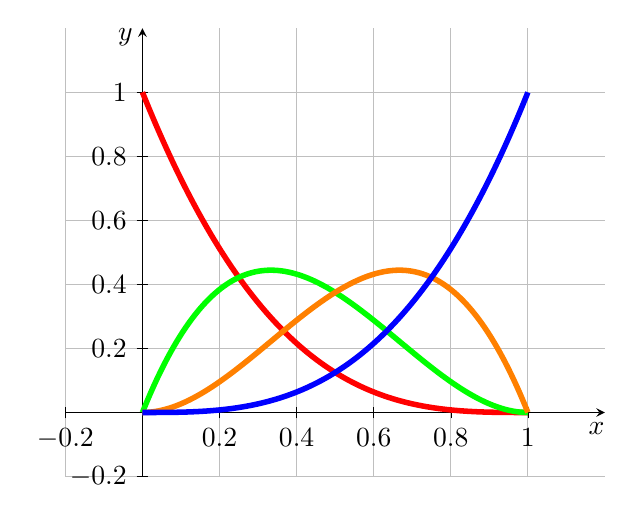
\begin{tikzpicture}[scale=1.0,
   declare function={  B30(\x)   =pow(1-\x,3); 
                       B31(\x)   =3*\x*pow(1-\x,2);
                       B32(\x)   =3*\x*\x*pow(1-\x,1);
                       B33(\x)   =pow(\x,3); 
                    },domain=0:1,smooth]
  \begin{axis}[
%      width=6cm,height=6cm,
      axis lines=middle,
      domain=0:1,
      smooth,
      no markers,
      grid,
      xmin=-0.2,xmax=1.2,
      tick style=black,
      xtick={-0.2,0,...,1},
      xlabel=$x$,
      xlabel style={below, anchor=north east,inner xsep=0pt},
      restrict y to domain=0:1,
      ymin=-0.2,ymax=1.2,
      ytick={-0.2,0,...,1},
      ylabel=$y$,
      ylabel style={above,anchor=north east,inner ysep=0pt},
      samples=100,
    ]
    \addplot[red,line width=2pt]{B30(\x)};
    \addplot[green,line width=2pt]{B31(\x)};
    \addplot[orange,line width=2pt]{B32(\x)};
    \addplot[blue,line width=2pt]{B33(\x)};
  \end{axis}

    \end{tikzpicture} 
  \caption{Bernstein-Polynom vom Grad $3$}
  \end{center}
\end{figure}

\bigskip

\DEF{
  Gegeben seien die Punkte 

  $$
	Q_{i} =	\left(
	\begin{array}{c}
	x_{i} \\
	y_{i}
	\end{array}
	\right) \quad \hbox{mit} \quad Q_{i} \in \R^2, \quad i = 0, 1, \ldots, n
  $$	
	
  Eine \textbf{Bézier-Kurve} ist dann definiert durch
	
  \begin{equation}
	C(\lambda) = \sum_{i=0}^n Q_{i}\cdot  b_{i,n}(\lambda)
	\label{Bezierkurve}
  \end{equation}
	
  Die Punkte $Q_i, i=0, \ldots, n$ heißen \textbf{Kontrollpunkte}.	
}	
	
\bigskip

Die Kontrollpunkte einer Bézier-Kurve bilden das sogenannte Kontrollpolygon.

\bigskip

\Bemerkung{
  Es sei der Startpunkt $P_0$ und der Endpunkt $P_1$, sowie die Tangenten $\vec{t}_0$ und $\vec{t}_1$ gegeben. Die Tangenten sind nicht notwendigerweise normiert.
  
  Die Kontrollpunkte  $Q_{0},Q_{1}, Q_{2}$ und $Q_{3}$ der zugehörigen Bézier-Kurve  sind durch folgende Gleichungen gegeben:

  \begin{equation}
    Q_{0}=P_{0},
    \qquad    
    Q_{1}=P_{0}+\lambda_{0} \vec{t}_{0},  
    \qquad   
    Q_{2}=P_{1}-\lambda_{1} \vec{t}_{n}, 
    \qquad    
    Q_{3}=P_{1}
	\label{KPunkte4}
  \end{equation}

  \cite{Jaklic:2010}	
}



\bigskip

\BEISPIEL{ \label{KPunkte4Beispiel}
  Gegeben seien
  $$
    P_0 = \binom{2}{4}, 
    \quad
    \vec{t}_0 = \binom{1}{1}
    \quad \hbox{und} \quad 
    P_1 = \binom{6}{1},
    \quad
    \vec{t}_1= \binom{1}{-2}
  $$    
  
  Dann ergibt sich gemäß Satz \ref{KPunkte4}   für Kontrollpunkte der zugehörigen Bézier-Kurve:
  
  $$
    Q_{0}=P_{0} = \binom{2}{4},
    \qquad    
    Q_{1}=P_{0}+\vec{t}_{0}
     = \binom{2}{4}+\binom{1}{1}=\binom{3}{5},  
  $$
  
  $$  
    Q_{2}=P_{1}- \vec{t}_{n}
         = \binom{6}{1} -\binom{1}{-2} = \binom{5}{3} , 
    \qquad    
    Q_{3}=P_{1} = \binom{6}{1}
  $$
 
  Die Bézier-Kurve und ihre Kontrollpunkte sind in der   Abbildung \ref{KPunkte4Graph} dargestellt. 
}
  
\begin{figure}
  \begin{center}
   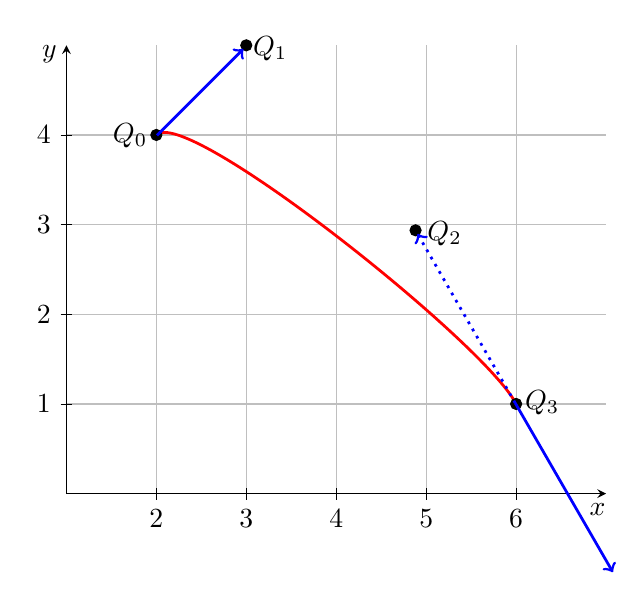
\begin{tikzpicture}[scale=1.0,
   declare function={  FX(\x)   =-6*pow(\x,3)+9*pow(\x,2)+\x+2; 
                       FY(\x)   = 5*pow(\x,3)-9*pow(\x,2)+\x+4; 
                    },domain=0:1,smooth]
  \begin{axis}[
%      width=6cm,height=6cm,
      axis lines=middle,
      domain=0:1,
      smooth,
      no markers,
      grid,
      xmin=1,xmax=7,
      tick style=black,
      xtick={1,2,...,6},
      xlabel=$x$,
      xlabel style={below, anchor=north east,inner xsep=0pt},
      restrict y to domain=-12:12,
      ymin=0,ymax=5,
      ytick={0,1,...,4},
      ylabel=$y$,
      ylabel style={above,anchor=north east,inner ysep=0pt},
      samples=100,
    ]
    \addplot[red,line width=1.0pt] ({FX(\x)}, {FY(\x)});
    \addplot[color = black,
    fill  = black,only marks] plot coordinates {(2,4) (6,1)
    ({2+1.414*cos(45)},{4.+1.414*sin(45)})
    ({6-2.236*cos(-60)},{1-2.236*sin(-60)}) };
    
    
  \end{axis}

    \coordinate[label=left:$Q_0$]  (P0) at (1.15,4.55);
    \coordinate[label=right:$Q_3$]  (P1) at (5.7,1.15);

    \coordinate[label=right:$Q_1$]  (P0T) at ({1.15+1.55*cos(45)},{4.55+1.55*sin(45)});
    \coordinate  (P1T) at ({5.7+2.48*cos(-60)},{1.15+2.48*sin(-60)});
    \coordinate[label=right:$Q_2$]  (P1Tn) at ({5.7-2.48*cos(-60)},{1.15-2.48*sin(-60)});
    
    \draw [blue,line width=1.0pt,->] (P0) -- (P0T);
    \draw [blue,line width=1.0pt,->] (P1) -- (P1T);
    \draw [blue,line width=1.0pt,->,dotted] (P1) -- (P1Tn);

    

    \end{tikzpicture} 
  \end{center}
  \caption{Bézier-Kurve zum Beispiel \ref{KPunkte4Beispiel} }
  \label{KPunkte4Graph}
\end{figure}
